\subsection{Mesh generation}
\label{sec:mesh_generation}

After having defined all the data of the problem in adequate data structures, the next step is to generate the mesh.
Generating a mesh means to discretize the domain into a finite number of elements, creating a grid of locations at which we will evaluate the approximate solution of the problem.

In particular, the algorithm has to return the following data structures:

\begin{itemize}
    \item \texttt{coordinates}: a matrix of size $N_{MeshNodes} \times N_{DoF}$ containing the $(x, y)$ coordinates of the nodes of the mesh.
    \item \texttt{connectivity}: a matrix of size $N_{Element} \times N_{NodesPerElement}$ containing the indices of the nodes that belong to each element of the mesh.
\end{itemize}

Moreover, we can analyze an example of mesh generation applied to a simple domain 2D domain composed of 2 rectangular-4-nodes elements, as shown in Figures \ref{fig:grid}, \ref{fig:node_numbering}, and \ref{fig:element_numbering}.

\begin{figure}[H]

    \begin{minipage}[b]{0.3\textwidth}
        \centering
        \begin{tikzpicture}
            \draw[step=2cm, gray, very thin] (0,0) grid (4,2);
            \draw[thick,->] (0,0) -- (4.5,0) node[anchor=north west] {x};
            \draw[thick,->] (0,0) -- (0,2.5) node[anchor=south east] {y};

            \foreach \x in {0,1,2}
            \draw (2*\x cm, 1pt) -- (2*\x cm,-1pt) node[anchor=north] {$\x$};

            \foreach \y in {0,1}
            \draw (1pt, 2*\y cm) -- (-1pt, 2*\y cm) node[anchor=east] {$\y$};
        \end{tikzpicture}
        \caption{Grid structure}
        \label{fig:grid}
    \end{minipage}
    %
    \hfill
    %
    \begin{minipage}[b]{0.3\textwidth}
        \centering
        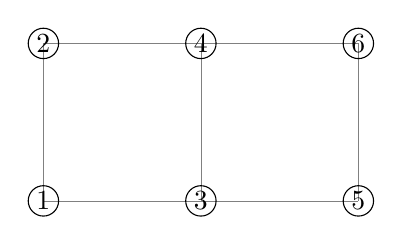
\begin{tikzpicture}
            \draw[step=2cm, gray, very thin] (0,0) grid (4,2);

            \foreach \x in {0,1,2}
                {
                    \foreach \y in {0,1}
                    \node[circle, draw, inner sep=1pt] at (2*\x cm, 2*\y cm) {$\the\numexpr2*\x+\y+1\relax$};
                }
        \end{tikzpicture}
        \caption{Node numbering (global indices)}
        \label{fig:node_numbering}
    \end{minipage}
    %
    \hfill
    %
    \begin{minipage}[b]{0.3\textwidth}
        \centering
        \begin{tikzpicture}
            \newcounter{elemindex}
            \setcounter{elemindex}{0}

            \draw[step=2cm, gray, very thin] (0,0) grid (2,2);

            \foreach \x/\y in {0/0,1/0,1/1,0/1}
                {
                    \node[circle, draw, inner sep=1pt] at (2*\x cm, 2*\y cm) {$\the\numexpr\value{elemindex}+1\relax$};
                    \stepcounter{elemindex}
                }
        \end{tikzpicture}
        \caption{Element numbering (element indices)}
        \label{fig:element_numbering}
    \end{minipage}

    \label{fig:example}

\end{figure}


At code level, all the information about the mesh numbering and space discretization are stored separately in the \texttt{coordinates} and \texttt{connectivity} matrices as follows:

\begin{table}[H]
    \centering
    \begin{tabular}{|c|cc|}
        \hline
        \textbf{Node index (global)} & \textbf{X (m)} & \textbf{Y (m)} \\
        \hline
        1                            & 0.0            & 0.0            \\
        2                            & 0.0            & 1.0            \\
        3                            & 1.0            & 0.0            \\
        4                            & 1.0            & 1.0            \\
        5                            & 2.0            & 0.0            \\
        6                            & 2.0            & 1.0            \\
        \hline
    \end{tabular}
    \caption{Coordinates matrix for the example above.}
    \label{tab:coordinates}
\end{table}

\begin{table}[H]
    \centering
    \begin{tabular}{|c|cccc|}
        \hline
        \textbf{Element index} & \textbf{\#1} & \textbf{\#2} & \textbf{\#3} & \textbf{\#4} \\
        \hline
        1                      & 1            & 3            & 4            & 2            \\
        2                      & 3            & 5            & 6            & 4            \\
        \hline
    \end{tabular}
    \caption{Connectivity matrix for the example above (\#n refers to the element node index).}
    \label{tab:connectivity}
\end{table}

Once the mesh has been generated, the next step is to compute the elemental matrices (in both the matrix and voigt form as needed).

